\scanpage{178}
% archive sheet number: 177
\figure{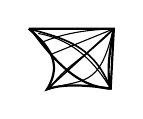
\begin{tikzpicture}[x=1cm,y=1cm]
\draw[thick] (0,.78) -- (1.08,.78) -- (1.04,.02) .. controls (.77,.06) and (.44,.09) .. (.23,.01)
 .. controls (.46,.37) and (.20,.61) .. (0,.78);
\draw[semithick] (0,.78) .. controls (.49,.65) and (.83,.55) .. (1.04,.02);
\draw[thick] (.03,.77) .. controls (.34,.35) and (.63,.04) .. (1.04,.02);
\draw (.12,.72) .. controls (.59,.64) and (.86,.32) .. (1.04,.02);
\draw (.17,.61) .. controls (.46,.73) and (.77,.77) .. (1.08,.78);
\draw (.27,.45) -- (1.08,.78); \draw[semithick] (.23,.01) -- (1.08,.78);
\draw (.26,.01) .. controls (.43,.29) and (.72,.41) .. (1.08,.78);
\draw (.23,.01) .. controls (.69,.15) and (.90,.02) .. (1.07,.77);
\draw[thick] (1.04,.02) .. controls (.97,.27) and (1.06,.65) .. (1.08,.78);
\end{tikzpicture}}

\[
\mathscr{E}xt^i(F,G)
\]

\[
\unsure{F_2|F_\ell|\deleted{F}}\qquad DG
\]

\[
\begin{aligned}
\mathbb R\mathscr{H}om(F,G)&\unsure{=|\simeq}\mathbb R\mathscr{H}om(F,DDG)\\
&\simeq\mathbb R\mathscr{H}om(F_{\unsure{,|1|\,}}\overset{\mathbb L}{\otimes}DG,R_X^\bullet)
\end{aligned}
\]

\[
F_{\unsure{1|<|\,}}\otimes DG
\]

\figure{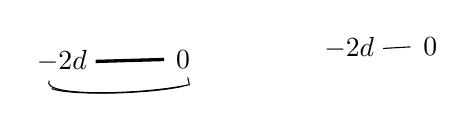
\begin{tikzpicture}[x=1cm,y=1cm]
\node at (0,0) {$-2d$}; \draw[very thick] (.43,-.005) -- (1.30,.02); \node at (1.54,.02) {$0$};
\draw (-.16,-.25) .. controls (-.27,-.46) and (1.03,-.43) .. (1.62,-.30) -- (1.60,-.21);
\draw (-.13,-.35) .. controls (.11,-.44) and (1.08,-.42) .. (1.54,-.32);
\node at (3.65,.17) {$-2d$}; \draw (4.08,.16) -- (4.43,.18); \node at (4.68,.18) {$0$};
\end{tikzpicture}}

\[
\deleted{\mathscr{E}xt^{i}}\qquad\mathscr H_i(F\otimes DG)\qquad\text{de }\dim\leq i
\]

\[
\mathscr{E}xt^i(F,G)\qquad D(F\overset{\mathbb L}{\otimes}DG
\]

\[
\boxed{\mathrm{Ext}^{\unsure{+|*}}(F_{\unsure{1|,|\,}},G)\Leftarrow E_1^{pq}=\mathrm{Ext}^{p\deleted{\unsure{+q|-q}}}(F\otimes\mathscr{E}xt^{-q}(G,A_X),A_X)}
\]

\figure{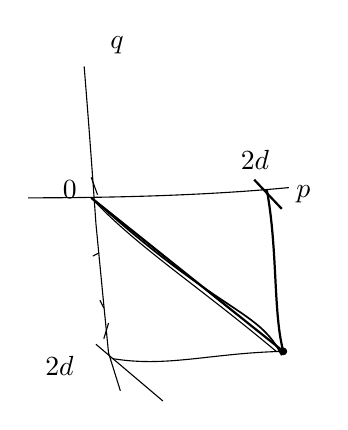
\begin{tikzpicture}[x=1cm,y=1cm]
\draw (-.8,0) .. controls (.10,0) and (1.36,.02) .. (2.51,.13);
\draw (-.09,1.67) .. controls (-.03,.94) and (.03,.10) .. (.06,-.33)
 -- (.15,-1.26) -- (.22,-1.97) -- (.37,-2.45);
\draw[thick] (2.23,.10) .. controls (2.37,-.65) and (2.31,-1.48) .. (2.44,-1.95);
\draw (.26,-2.04) .. controls (.96,-2.16) and (1.52,-1.97) .. (2.44,-1.95);
\draw[thick] (0,0) -- (2.44,-1.95);
\draw (0,0) .. controls (.58,-.62) and (1.31,-1.08) .. (2.35,-1.95);
\draw[semithick] (.04,-.03) .. controls (1.68,-1.50) and (2.12,-1.41) .. (2.42,-2);
\draw (0,.26) -- (.08,.04); \draw (.02,-.74) -- (.1,-.70);
\draw (.16,-1.40) -- (.11,-1.30); \draw (.16,-1.79) -- (.22,-1.59);
\draw (.06,-1.86) -- (.91,-2.58);
\draw[thick] (2.07,.23) -- (2.42,-.14); \fill (2.44,-1.95) circle (1.4pt);
\node[above right] at (.12,1.7) {$q$}; \node[left] at (-.06,.11) {$0$};
\node[above] at (2.08,.24) {$2d$}; \node[right] at (2.48,.04) {$p$};
\node[left] at (-.10,-2.13) {$2d$};
\end{tikzpicture}}

\[
\deleted{\unsure{q^4-q|q^4-q^1|q^4=q}}\unsure{2q|\geq q}\qquad F\otimes\mathscr{E}xt^{2d}(G,A)
\]

\[
\deleted{\mathscr{E}xt^p(}
\]

$\operatorname{supp}\mathscr{E}xt^{-q}(G,A_X)$ de \deleted{\unsure{d|D}}codim $\geq-q$

\deleted{de dim $\leq$}

donc $\mathscr{E}xt^p(\ ,A_X)=0$ si $p\unsure{<|\leq}-q$ i.e. si $\unsure{pq|p+q}<0$

\[
\deleted{\mathscr{E}xt^*(}\qquad \mathscr{E}xt^{2d}(F,G)\simeq\mathscr{E}xt^{2d}(F\otimes\mathscr{H}om(G,A_X),A_X)
\]
